\documentclass[11pt,a4paper,ngerman]{article}
\usepackage[utf8]{inputenc}
\usepackage[T1]{fontenc}
% Times New Roman
\usepackage{newtxtext,newtxmath}
\usepackage[ngerman]{babel}

\usepackage{geometry}
\geometry{left=2.5cm, right=2.5cm, top=2.5cm, bottom=2cm}
\usepackage[onehalfspacing]{setspace}
\usepackage{graphicx}
\graphicspath{{img/}}
\usepackage{wrapfig}
\usepackage{caption}
\captionsetup{
  font=small,            
  labelfont=bf           
}
\usepackage{subcaption}
\captionsetup[subfigure]{skip=4pt}
\usepackage{enumitem}
\usepackage{listings}
\usepackage{xcolor}
\definecolor{mygreen}{rgb}{0,0.6,0}
\definecolor{mygray}{rgb}{0.5,0.5,0.5}
\definecolor{mymauve}{rgb}{0.58,0,0.82}
\lstset{
	keywordstyle=\color{blue},commentstyle=\color{mygreen},
	stringstyle=\color{mymauve},rulecolor=\color{black},
	basicstyle=\footnotesize\ttfamily,
	captionpos=b, % sets the caption-position to bottom
	keepspaces=true, % keeps spaces in text
	numbers=left, numbersep=5pt, showspaces=false,showstringspaces=true,
	showtabs=false, tabsize=2, title=\lstname
}
\lstdefinestyle{customc_compact}{
    language=C++,
    basicstyle=\scriptsize\ttfamily, % <-- WICHTIG: Kleinere Schriftart
    numbers=left,
    numberstyle=\tiny\color{gray},
    stepnumber=1,
    numbersep=5pt,
    breaklines=true,
    showstringspaces=false,
	frame=tb,
	framexleftmargin=5pt,
	backgroundcolor=\color{gray!5},
}
\usepackage{algorithm}
\usepackage{algpseudocode}
\algnewcommand{\Var}[1]{\mathit{#1}}
\algnewcommand{\Break}{\textbf{break}}
\algnewcommand{\True}{\textbf{true}}
\algnewcommand{\False}{\textbf{false}}
\MakeRobust{\Call}
\usepackage[backend=biber]{biblatex}
\addbibresource{bib.bib}
\DeclareNameAlias{default}{last-first}
\usepackage{amsmath}
\let\openbox\undefined
\usepackage{amsthm}
\usepackage{amstext}
\usepackage{pifont}
\theoremstyle{definition}
\newtheorem{definition}{Definition}[section]
\theoremstyle{plain}
\newtheorem{example}{Beispiel}
\newtheorem{theorem}{Theorem}[section]
\usepackage{booktabs}
\usepackage{array}
\renewcommand{\arraystretch}{1.1}
\usepackage{tabularx}
%\usepackage{lipsum}
% Muss immer letztes Packet sein
\usepackage{hyperref}
\usepackage{cleveref}

\title{\bf\Huge PoP: Probabilistische opake Prädikate gegen symbolische Ausführung}
\date{}

\begin{document}
\begin{titlepage}
	\centering
  	\maketitle
	\vfill
	\begin{tabular}{ll}
		Teilnehmende: & Paul Baumgartner (18 J.) \\
		Erarbeitungsort: & Hildesheim \\
		Projektbetreuende: & Dr. Arndt Latußeck\\
		Fachgebiet: & Mathematik/Informatik \\
		Wettbewerbssparte: & Jugend forscht \\
		Bundesland: & Niedersachsen \\
		Wettbewerbsjahr: & 2026 \\
	\end{tabular}
	\thispagestyle{empty}
\end{titlepage}

\thispagestyle{empty}
\section*{Projektüberblick}
%\textcolor{red}{TODO: Fachliche Kurzfasssung!!!}
Diese Arbeit beschäftigt sich damit, Computerprogramme so zu verändern, dass eine Rekonstruktion ihrer Programmlogik für Angreifer wirtschaftlich unrentabel ist. Hierfür wurde eine Methode entwickelt, die Bedingungen in Programmen einsetzt, um die Komplexität der Programme zu erhöhen, ohne dabei den Programmablauf zu verändern. Im Unterschied zu existierenden Methoden funktioniert diese über die Einbindung von Wahrscheinlichkeiten. Diese erschweren eine Entfernung der eingeführten Bedingungen und somit auch der Komplexität für Angreifer erheblich, wie durchgeführte Experimente belegen.

\newpage
\thispagestyle{empty}
\tableofcontents

\newpage
\setcounter{page}{1}

\section{Einleitung}
\emph{Obfuskation} (lat. \emph{obfuscare}: verdunkeln) bezeichnet jede Transformation von Programmen zur Hinderung von sog. Reverse Engineering - der Analyse von Software zum Cracken, Verstehen oder Kopieren.
Obfuskation kommt zum Einsatz in der Malwareentwicklung, in der Industrie und im Militär\cite{darpaSafeWare}. Da das Programm hierbei noch die ursprüngliche Semantik beibehält kann jede Software mit genügend Zeit, Aufwand und Geld trotz Obfuskation verstanden werden. Der Sinn von Obfuskation ist also nicht die komplette Verhinderung von \emph{Reverse Engineering}, sondern vielmehr dieses wirtschaftlich unrentabel zu machen.
Von besonderem Interesse im Bereich der Obfuskation sind opake Prädikate, eine Kontrollflussobfuskation welche immer wahre bzw. falsche Verzweigungen in Programme einfügt.

In dieser Arbeit wird folgender Frage nachgegangen: \emph{Ist es Möglich, opake Prädikate zu kreieren, welche eine automatisierte Deobfuskation mit aktuellen Methoden verhindern und dabei praxisgerecht bleiben?} Die Relevanz dieser Forschungsfrage ergibt sich aus dem fortdauernden Kampf zwischen Obfuskation und Deobfuskation sowie der Effektivität von symbolischer Ausführung gegen opake Prädikate.

Die Kernbeiträge dieser Arbeit hierzu sind folgende: 
\begin{itemize}
    \item Es wird das neue Konzept probabilistischer opaker Prädikate vorgestellt. Es handelt sich dabei um opake Prädikate, welche durch die Nutzung von Wahrscheinlichkeitsverteilungen und Pseudozufallsvariablen verschiedene Angriffsmethoden verhindern.
    \item Es wird ein Algorithmus geliefert, um mittels Bernsteinpolynomen probabilistische opake Prädikate mit zufälligen Wahrscheinlichkeitsverteilungen zu generieren. Der Algorithmus wird implementiert und erfolgreich evaluiert.
    \item Dabei wird ein Problem bei der Generierung symbolischer Variablen über Funktionsparameter angesprochen und \cref{alg:symVar} als Lösung präsentiert. 
    Nach bester Kenntnis des Autors handelt es sich hierbei um ein neuen undokumentierten Angriffsvektor.
\end{itemize}
In dieser Arbeit wird sich bewusst auf die Erzeugung der opaken Prädikate selbst beschränkt. Die Relevanz von Füllcode (sog. \emph{Junkcode}) ist unabhängig von den dargestellten Idee und wird daher nicht behandelt.
Zunächst werden Obfuskation, opake Prädikate und symbolische Ausführung formal definiert (\cref{sec:theorie}). Durch einen Überblick über den aktuellen Stand der Forschung (\cref{sec:motivation}) wird die Notwendigkeit dieser Arbeit hergeleitet und ein Angreifermodell festgelegt (\cref{sec:angreiferModell}).
In \cref{sec:probOpak}-3 wird die Idee propabilistischer opaker Prädikate vorgestellt und definiert. Darauf werden verschiedene Methoden zur zufälligen Wahrscheinlichkeitsverteilungsgenerierung (\cref{sec:genProb}) sowie zur Generierung von Pseudozufallszahlen (\cref{sec:pseudoZufall}) vorgestellt und abgewogen. Dabei wird das bis jetzt nicht untersuchte Problem der Aufruf-Invarianz für die Generierung symbolischer Variablen über Funktionsparameter angesprochen und über \cref{alg:symVar} gelöst.
Implementiert wird die Idee in Form eines LLVM-Passes (\cref{sec:implementierung}). 
Eine Evaluierung anhand der Kriterien Collbergs et al. \cite{collbergATaxonomyOfObfuscatingTransformations} (\cref{sec:evaluierung}) zeigt, dass probabilistische opake Prädikate resilient gegenüber symbolischer Ausführung und weiteren Methoden sind, ohne dabei unvertretbare Kosten aufzuweisen.

Diese Arbeit geht von einem informatischen Grundwissen an Assembler, Compilern sowie Programmanalysemethoden aus. Zudem wird die Iverson-Klammer/ Prädikatabbildung $[\cdot]$ verwendet: Unter der Voraussetung, dass die Aussage $P$ wahr ist, gilt $[P]=1$. Ansonsten gilt $[P]=0$. Pseudocode, welcher Programmanweisungen modifiziert nimmt an, dass diese in \emph{Single Static Asignment}-Form definiert sind.
%Vergleicht eine Aussage zwei Variablen, so wird hierfür "`$==$"' verwendet.
%\textcolor{red}{TODO: Klären, was in welchem Abschnitt gemacht wird}

\section{Theoretische Grundlagen} \label{sec:theorie}
\subsection{Obfuskation}
Collberg et al. \cite{collbergATaxonomyOfObfuscatingTransformations} definieren Obfuskation wie folgt:
\begin{definition}[Obfuskation]
	Sei $P \xrightarrow{\mathcal{T}}P'$ eine Transformation $\mathcal{T}$ eines \emph{Quellprogrammes} $P$ zu einem \emph{Zielprogramm} $P'$.
	Eine solche Transformation ist eine Obfuskation, wenn das obfuskierte Programm $P'$ dasselbe beobachtbare Verhalten wie $P$ für den Endnutzer aufweist.  %\textcolor{red}{TODO: Barak et al. nutzen!}
\end{definition}

Obfuskation zielt darauf ab, die Komplexität eines Programmes so zu erhöhen, dass dessen interne Logik für einen Angreifer nur schwer verständlich ist. %Für die Komplexität von Programmen gibt es mehrere Metriken \cite{collbergManufacturingCheapResilient1998}. Näheres hierzu folgt in \cref{sec:kriterien}.
Per Definition sind Nebenwirkungen (z.B. Herunterladen von neuen Daten etc.) erlaubt, solange sie nicht vom Nutzer erfahren werden. Die präsentierte Methode dieser Publikation nutzt diese Lockerung der Einschränkungen auf obfuskierende Transformationen aus, wie später ersichtlich sein wird.

Das Rückgängigmachen einer Obfuskation ist die \emph{Deobfuskation}.

\subsection{Opake Prädikate}
Die folgenden Definitionen sind aus \cite{tofighi-shiraziDefeatingOpaquePredicates2019} sowie vom Pionierwerk \cite{collbergManufacturingCheapResilient1998} modifiziert übernommen. Es wird sich auf hierbei auf invariante opake Prädikate beschränkt.
\begin{definition}[Opake Prädikate]
	Sei $\mathcal{O} : \Phi \rightarrow \{0, 1\}$ eine Abbildung einer Variable $\phi\in \Phi$ zu einem Prädikat. Das Prädikat $\mathcal{O}(\phi)$ ist opak, wenn für alle $\phi\in \Phi$ gilt, dass $\mathcal{O}(\phi)$ denselben Wert ($1$ oder $0$ bzw. wahr oder falsch) hat.
\end{definition}
In anderen Worten: Das Prädikat $\mathcal{O}(\phi)$ ist opak, wenn dessen Wert für alle möglichen Parameter \emph{a priori} bestimmt ist (also für den Programmierer bekannt ist) aber für ein Verständnis einer weiteren Person (ein Angreifer) \emph{a posteriori} (durch Beobachtung) zu bestimmen ist \cite{collbergManufacturingCheapResilient1998}.

\begin{minipage}[t]{0.45\textwidth}
  \centering
  \includegraphics[ 
    scale=1.25
    ]{overwatch_byfron_cropped}
  \captionof{figure}{Kontrollflussgraph einer einfachen Funktion mit opakem Prädikat. %Abbildung aus der Disassembly des Spiels \emph{Overwatch} mittels IDA entnommen.
  } \label{fig:overwatchGraph}
\end{minipage}\hfill
\begin{minipage}[t]{0.5\textwidth}
  \centering
  % \resizebox{\columnwidth}{!}{\usebox{\idacode1}}
  \includegraphics[scale=0.2]{komplex_cropped}
  \captionof{figure}{Ausschnitt des Kontrollflussgraphen einer Funktion mit vielen opaken Prädikaten. Durch die vielen opaken Prädikate wird die Funktion unübersichtlich und eine Analyse aufgrund der Unklarheit tatsächlich ausführbarer Pfade erschwert. %Abbildung aus der Disassembly des Spiels \emph{Overwatch} mittels IDA entnommen.
  } \label{fig:overwatchGraph2}
\end{minipage} \\

Opake Prädikate werden in der Softwareobfuskation eingesetzt, um ein Verständnis über den Kontrollfluss des Programms zu behindern \cite{collbergManufacturingCheapResilient1998, tofighi-shiraziDefeatingOpaquePredicates2019}. Damit opake Prädikate als Obfuskationsmethode \footnote{D.h, dass der wirkiche Pfad, welcher von einem opaken Prädikat verschleiert wird, nicht einfach erkannt werden kann} genutzt werden können, müssen sie wiederholt angewandt werden. Dadurch entsteht ein komplexerer Kontrollflussgraph und der Angreifer weiß folglich nicht, welche Basisblöcke zu analysieren sind. Die Stärke der opaken Prädikate ist hierbei abhängig von der Stärke ihres Terms/Ausdrucks \cite{collbergManufacturingCheapResilient1998}. Mit zunehmender Komplexität der Prädikate und zunehmender Anzahl dieser, nimmt also auch die Obfuskationsstärke (Verwirrung und Unverständnis) beim Angreifer zu (vgl. \cref{fig:overwatchGraph2}).

\begin{example}
Das Prädikat $\mathcal{O}(\phi)=\left[-1977224191 \space \& \space 1 = 1\right]$ aus \cref{fig:overwatchGraph}, wobei "`$\&$"' dem bitweisen "`und"' Operator entspricht, ist sehr einfach. Eine Berechnung genügt, um zu erkennen, dass das Prädikat immer wahr ist.
\end{example}

\begin{example}
Das Prädikat $\mathcal{O}(\phi)= \left[(y < 10) \vee (x \cdot (x + 1) \mod{2} \equiv 0)\right]$ aus \text{\cite{ieeespro2015-JunodRWM}} mit $\phi=(x,y)$ und $x, y \in \mathbb{Z}$ ist immer wahr, da $x\cdot (x+1)$ immer gerade ist. Der Wert is folglich von $y$ unabhängig.
\end{example}

\subsection[Symbolische Ausführung]{Symbolische Ausführung\footnote{Die Angaben des folgenden Abschnitts entstammen, sofern nicht anders vermerkt, aus \cite{baldoniSurveySymbolicExecution2018}}} % Automatische Deobfuskationsattacken
Im Gegensatz zur konkreten Ausführung, welche ein Programm für spezifische Inputs ausführt, ermöglicht die symbolische Ausführung die Analyse des Programmverhaltens für ganze Klassen an Inputs.
Die Notwendigkeit symbolischer Ausführung ergibt sich schon am Beispiel einer einer Funktion mit zwei 64-Bit Variablen. Um mit dynamischer (konkreter) Ausführung herauszufinden, für welche Werte eine Bedingung wahr ist, müsste man hier $2^{64} \cdot 2^{64} = 2^{128}$ verschiedene Werte ausprobieren. Ein solcher Bruteforce ist selbst für die modernsten Computer unmöglich - symbolische Ausführung hingegen schon.
Ein symbolischer \emph{Ausführungsengine} besteht aus 2 Hauptkomponenten: einem \emph{symbolischen Ausführungsmodul} und einem \emph{Constraint-Solver}\footnote{Es handelt sich meist um einen SMT-Solver.} zur Lösung/zum Prüfen von Bedingungen/Einschränkungen. 
Bei der symbolischen Ausführung wird für jeden Kontrollflussweg eine \emph{Pfadformel} und ein \emph{symbolischer Speicher} mitgeführt. 
\begin{enumerate}[]
	\item Die Pfadformel, eine boolesche Formel erster Ordnung, führt die Bedingungen der entlang des Pfades genommenen Verzweigungen zusammen. 
	\item Der symbolische Speicher bildet unbekannte Variablen (z.B. Parameter und alle darauf aufbauende Variablen) auf symbolische Ausdrücke ab.
\end{enumerate}
Hierdurch können schließlich über den \emph{Constraint-Solver} allgemeine Aussagen über die Erreichbarkeit bestimmter Pfade oder Variablenwerte getroffen werden. Ist eine Pfadformel erfüllbar, kann der Solver zudem konkrete Eingebewerte hierfür liefern.
Hat das Programm aber besonders viele Verzweigungen (z.B. durch Schleifen) oder komplexe Constraints (z.B. nichtlineare Arithmetik), stoßen die \emph{Constraint-Solver} an ihre laufzeittechnischen Grenzen. Zur Lösung wurden verschiedene Ansätze (z.B. \emph{Concolic Execution}) entwickelt. Aufgrund der Fülle an Informationen und der geringen Relevanz für die in dieser Arbeit dargestellten Abwehrmethodik, wird auf ihre Darstellung verzichtet.

\section{Stand der Forschung und Motivation} \label{sec:motivation}
Dieser Abschnitt präsentiert den aktuellen Stand der Forschung zu opaken Prädikaten und begründet daraus diese Arbeit. Es werden aktuelle, zentrale Ansätze exemplarisch vorgestellt, um Forschungsstand und Herausforderungen zu verdeutlichen. Die geschieht anhand der Kriterien aus \cref{sec:kriterien}.

Existierende Literatur beschränkt sich vornehmlich auf statische Analyseansätze. Dynamische Analyseideen z.B. zur probabilistischen Untersuchung opaker Prädikate wurden veröffentlicht und experimentell untersucht, ergaben aber eine zu hohe Fehlerquote. Insbesondere reduzieren sich publizierte Ansätze auf symbolische Ausführung. Dies hat den Hintergrund, dass die symbolische Ausführung momentan eine der effektivsten automatisierten Analysemethoden bildet, welche mit wenig Aufwand und eigenem Eingriff verwendet werden kann. Andere Analysemethoden, wie z.B. \emph{Tainting} sind zudem abhängiger von Faktoren neben den opaken Prädikaten selbst. Im Falle des \emph{Taintings} ist die Qualität des Füllcodes wesentlich \cite{zobernigWhenAreOpaque2019}.

%Trotz der Effektivität mancher existierender Methoden, bleiben viele formal unbegründet. Ihre Resistenz basiert auf Implementierungsschwächen\footnote{bzw. Heuristikschwächen.} existierender symbolischer Ausführungsengines und nicht ihren fundamentalen Grenzen (bzw. den der Constraint-Solver) \cite{xuManufacturingResilientBiOpaque2018}. Als Beispiel hierfür dienen die Bi-Opaken Prädikate \cite{xuManufacturingResilientBiOpaque2018}. Eine Befragung von Audrey Dutcher, einer der Entwicklerinnen von \emph{Angr} \cite{shoshitaishvili2016state} ergab: drei der vier in \cite{xuManufacturingResilientBiOpaque2018} dargestellten Methoden können nun von \emph{Angr} problemlos symbolisch ausgeführt werden
%\footnote{
%	(a) symbolischer RAM: Ausführbar für Arrays mit einer Länge unter $257$. \\
%	(b) Gleitkommazahlen: Ausführbar, wenn keine x86 \texttt{long double} Datentypen verwendet werden. \\
%	(c) Verdeckte symbolische Kontrollflussübertragung (\emph{Covert Symbolic Propagation}), in \cite{xuManufacturingResilientBiOpaque2018} über Dateisystem-Operationen implementiert: Ausführbar. \\
%	(d) Threads: Noch nicht implementiert.
%}.
%Die Deobfuskation weiterer Methoden wie \cite{linBranchObfuscationUsing2013}, \cite{tigress2025} und \cite{linBranchObfuscationUsing2013} liegt also alleine in der Verbesserung existierender symbolischer Ausführungsengines.
%Eine Deobfuskation ist in gewisser Weise nur eine Frage der Zeit.
%
%Andere Methoden, wie \cite{wangLinearObfuscationCombat2011} und \cite{ogisoSoftwareObfuscationTheoretical2003} sind zwar formal sicher, sind aber einfach erkennbar und weisen hohe Laufzeitkosten auf.
Existierende Methoden lassen sich im Wesentlichen in zwei Kategorien einteilen:

\begin{enumerate}
    \item Opake Prädikate, welche Implementierungsschwächen\footnote{bzw. Heuristikschwächen.} existierender symbolischer Ausführungsengines angreifen. 
    
    Hierunter fällt die Nutzung von \emph{Exceptions} \cite{linBranchObfuscationUsing2013}, Anweisungen \cite{xuManufacturingResilientBiOpaque2018} oder Funktionen \cite{tigress2025}, welche nicht durch die symbolischen Ausführungsengines modelliert werden.
Eine Befragung von Audrey Dutcher, einer der Entwicklerinnen vom Programmanalyseframework \emph{Angr} \cite{shoshitaishvili2016state} ergab: drei der vier in \cite{xuManufacturingResilientBiOpaque2018} dargestellten Methoden können nun von dem symbolischen Ausführungsengine von \emph{Angr} problemlos symbolisch ausgeführt werden
\footnote{
    	(a) symbolischer RAM: Ausführbar für Arrays mit einer Länge unter $257$. \\
    	(b) Gleitkommazahlen: Ausführbar, wenn keine x86 \texttt{long double} Datentypen verwendet werden. \\
    	(c) Verdeckte symbolische Kontrollflussübertragung (\emph{Covert Symbolic Propagation}), in \cite{xuManufacturingResilientBiOpaque2018} über Dateisystem-Operationen implementiert: Ausführbar. \\
    	(d) Threads: Noch nicht implementiert.
}.Eine Deobfuskation weiterer Methoden in dieser Kategorie liegt also alleine in der Verbesserung existierender symbolischer Ausführungsengines. Eine Deobfuskation ist in gewisser Frage nur eine Frage der Zeit.

    \item Opake Prädikate, welche fundamentale Grenzen der \emph{Constraint Solver} angreifen.
    
    Diese Nutzen entweder ungelöste Probleme in der Mathematik oder NP-schwere Probleme der Informatik. So erstellte \cite{wangLinearObfuscationCombat2011} z.B. opake Prädikate, welche auf der unbewiesenen Vermutung basieren, dass die Collatz Folge unabhängig vom Startwert immer den Zyklus $4,2,1$ erreicht. Da Mathematiker noch nicht die Werkzeuge haben, dies zu beweisen, ist die symbolische Ausführung auch nicht in der Lage zu beweisen, dass das Programm weiterläuft und nicht in eine Endlosschleife gerät. In \cite{ogisoSoftwareObfuscationTheoretical2003} wird alternativ ein NP-schweres Problem mit Pointerarithmetik konstruiert. In beiden Fällen sind die opaken Prädikate zwar beweisbar sicher, allerdings einfach erkennbar und mit hohen Laufzeitkosten verbunden. Andere Methoden wie opake Prädikate mit \emph{Mixed Boolean Arithmetic} Ausdrücken lassen sich mit neusten Heuristiken mitlerweile trotz NP-schwere größtenteils deobfuskieren \cite{reichenwallnerSimplificationGeneralMixed2023}.
\end{enumerate}

%Angesichts der Schwierigkeiten aktueller Methoden ergibt sich die Notwendigkeit effizienter, getarnter und resilienter (nur schwer automatisch deobfuskierbarer) opaker Prädikate.
Angesichts der dargelegten Probleme aktueller Methoden ergibt sich die Notwendigkeit effizienter, getarnter und resilienter (nur schwer automatisch deobfuskierbarer) opaker Prädikate.

\section{Ansatz} 
\subsection{Angreifermodell} \label{sec:angreiferModell}
Diese Arbeit geht aufgrund der Ähnlichkeit behandelter Thematik von einem \emph{Man-at-the-End} (MATE) Angreifermodell aus, aufbauend auf \cite{xuManufacturingResilientBiOpaque2018, zobernigWhenAreOpaque2019}.
Ein Angreifer hat direkten Zugriff auf das Programm und dessen Anweisungen sowie volle Kontrolle über das Endsystem, auf dem sie ausgeführt werden. 
\begin{wrapfigure}{r}{0.3\textwidth}
	\centering
	\includegraphics[width=0.3\textwidth]{sym_exec}
	\caption{\centering Konzeptionelles Framework zur Erkennung opaker Prädikate mit symbolischer Ausführung. Abbildung aus \cite{xuManufacturingResilientBiOpaque2018} übernommen.} 
\end{wrapfigure}
Es ist dem Angreifer hierbei nicht vorgegeben, wo und inwiefern das Programm obfuskiert ist. Der Angreifer kann das Programm statisch und dynamisch analysieren. Das Ziel des Angreifers ist dabei, ein Verständnis der obfuskierten Programmlogik zu gewinnen.
%Der Angreifer kann das Programm nur statisch analysieren. Der Angreifer kann das Programm nicht im vollen Ganzen dynamisch ausführen. Solchen Situationen begegnet man z.B. bei Malware, welche gegen Virtuelle Maschinen (\emph{virtual machines}) gehärtet ist oder bei Software, welche für proprietäre und unverfügbare Systeme geschrieben ist.
Pattern Matching, also das Suchen von Assembler-Anweisungsfolgen, kann hierbei zum Finden und Löschen zuvor erkannter opaker Prädikate verwendet werden. 
Zudem kann der Angreifer Funktionen symbolisch ausführen. Über eine Anfrage an den Constraint-Solver kann hierbei geprüft werden, ob ein Prädikat für alle Eingabewerte wahr ist. Ist dies der Fall, so handelt es sich um ein opakes Prädikat, welches gelöscht werden kann.
Mögliche dynamischer Analysemethoden werden in \cref{sec:fazit} angeführt und diskutiert.

\subsection{Probabilistische opake Prädikate} \label{sec:probOpak}
Symbolische Ausführung genügt für die Untersuchung deterministischer Algorithmen und entscheidbarer Probleme.
Will man aber Aussagen über einen probabilistischen Algorithmus treffen, so ist dies ohne erhebliche manuelle Eingriffe eines Nutzers in Form von extra Annahmen und Beschränkungen (\emph{Constraints}) unmöglich. Jede zufällige Variable eines jeden Schleifenaufrufes muss vom Constraint Solver als symbolische Variable betrachtet und das Programm für alle möglichen Werte untersucht werden. Bei einem Monte-Carlo-Algorithmus bedeutet dies, dass auch unwahrscheinliche Variablenwerte, welche zu falschen Ergebnissen führen, überprüft werden. Der Wahrheitsgehalt wird somit zwar formal logisch korrekt bewiesen - praktisch allerdings nicht.
\begin{example}
Man betrachte einen Algorithmus, welcher mit einer Wahrscheinlichkeit von $99,9999\%$ den Wert $1$ zurückgibt und mit einer Wahrscheinlichkeit von $0,0001$ den Wert $0$ zurückgibt. 
\begin{algorithm}[!htb] 
    \caption{Beispiel eines probabilistischen Algorithmus}
    \label{alg:bspProb1}
    \begin{algorithmic}[1]
    \Procedure{Foo}{{}}
        \State $\Var{X} \gets \Call{UniformRand}{0,1}$
        \If{$\Var{X} \leq 0,999999$}
            \State \Return $1$
        \EndIf
        \State \Return $0$
    \EndProcedure
    \end{algorithmic}
\end{algorithm}

Nutzt man einen symbolischen Ausführungsengine, um zu prüfen, ob der vorliegende Algorithmus den Wert $1$ wiedergibt, so würde dieser behaupten, dass dies falsch sei.
\end{example}

Dies bildet die Grundidee probabilistischer opaker Prädikate. Anstatt Prädikate zu bilden, welche für alle Werte ihrer Parameter \emph{wahr} bzw. \emph{falsch} sind, werden Prädikate erzeugt, deren gewünschter Wert so wahrscheinlich ist, dass das Gegenteil praktisch nie auftritt.
\begin{definition}[Probabilistische opake Prädikate] \label{def:probOpaque} \label{def:konstruktionsschema}
	Sei $\mathcal{O}_p : \Phi \rightarrow \{0, 1\}$ eine Abbildung einer Variable $\phi\in \Phi$ zu einem Prädikat. Das Prädikat $\mathcal{O}_p(\phi)$ ist probabilistische opak, wenn der Fall $A\in \{0, 1\}$ mit einer so hohen Wahrscheinlichkeit eintritt, dass der Fall $\overline{A}$ vernachlässigbar ist. %\textcolor{red}{Formaler mit $\epsilon$ wie Barak et al.?}
\end{definition}

\begin{definition}
	Sei $X$ eine Zufallsvariable mit beliebiger Wahrscheinlichkeitsverteilung $P(X; \theta)$, wobei $\theta$ die Parameter der Verteilung darstellt. Das probabilistische opake Prädikat $\mathcal{O}_p(\phi)$ wird wie folgt konstruiert:  
\begin{equation}
	\mathcal{O}_p(\phi) = \left[f(X) \bowtie c \right],
\end{equation}
	wobei:
	\begin{enumerate}
		\item $f$ eine Transformation durch arithmetische und bitweise Operationen ist (z. B. $f(X) = m \cdot (X \oplus k) + b$)), mit Konstanten $(m, k, b) \in \mathbb{R}$,
		\item $\bowtie$ ein Zahlenvergleichsoperator ist ($=$, $>$, $<$, $\geq$, $\leq$) und
		\item $c$ eine festgelegte Konstante ist.
	\end{enumerate}
\end{definition}
\begin{definition} \label{def:pProb}
	$\mathcal{P}_{\Var{prob}}$ ist die Klasse aller probabilistische opaker Prädikate.
\end{definition}

\begin{example} \label{ex:gleich}
	Ein einfaches probabilistisches opakes Prädikat ist $\mathcal{O}_p(\phi) = \left[\Call{Uniform}{0,1} \leq 1-10^{-2} \right]$. Die Wahrscheinlichkeit, dass dieses Prädikat wahr ist, beträgt $1-10^{-2}=0,99\%$.
\end{example}

\begin{example}
	$\mathcal{O}_p(\phi) = \left[\Call{Poisson}{5} \geq 15 \right]$. Die Wahrscheinlichkeit, dass dieses Prädikat unwahr ist beträgt $\sum_{k=15}^{\infty} \frac{5^ke^{-5}}{k!} = 1 - \sum_{k=0}^{14} \frac{5^ke^{-5}}{k!} \approx 0,023\%$
\end{example}

Um zu garantieren, dass das Programm, in welchem das probabilistische opake Prädikat eingefügt wurde, weiterhin funktioniert, kann für den ungewünschten Gegenfall eine Wahrscheinlichkeit genutzt werden, welche unter der eines Hardwarefehlers liegt. %Auch gewöhnliche Programme bzw. Computer können spontan versagen. Durch das Nutzen so geringer Wahrscheinlichkeiten \textcolor{red}{TODO ...}

Die geringe Wahrscheinlichkeit, dass die Prädikate in $\mathcal{P}_{\Var{prob}}$ sich nicht wie gewünscht verhalten, gewährleistet ihnen theoretische Resistenz gegenüber symbolischer Ausführung. Ohne Heuristiken ist es (bei adäquater Implementierung) theoretisch unmöglich, zwischen einem "`normalen"' Prädikat, welches besonders häufig einen Wert annimmt, und einem probabilistischen opaken Prädikat zu unterscheiden. (vgl. \cref{bspProb}) Dies zwingt den Angreifer zu einer genaueren Analyse jedes Prädikats im Sachzusammenhang.

\begin{example} \label{bspProb}
    Sei $p$ ein Prädikat, welches zu $95\%$ der Zeit wahr ist. Ist $p \in \mathcal{P}_{\Var{prob}}$ oder einfach besonders häufig wahr?
\end{example}

\subsection{Konstruktionsalgorithmus} \label{sec:alg}
\begin{algorithm}[!h] 
	\caption{Generierung probabilistischer opaker Prädikate}
	\label{alg:probOpaque}
	\begin{algorithmic}[1]
		\Require $\Var{D_{start}}, \Var{D_{end}}$ (Domain of inverse CDF), $P(\Var{TrueBB})$ (Probability of generated predicate having wanted value), $\Var{Precision}$ (determines $\Var{Threshold}$ precision in predicate)
		\Procedure{GenerateProbabilisticPredicates}{$\Var{Module}, \Var{CDF}, \Var{p} \in [0, 1], \Var{Precision} \in \mathbb{N}$}
		\For{$Function \; \Var{F} \in \Var{Module}$}
		\If{\Call{ShouldObfuscate}{$\Var{F}$}}
		\State $\Var{BB} \gets \Call{GetRandomBasicBlock}{\Var{F}}$
		
		\State $\Var{U} \gets \Call{GetSymbolicVariable}{$$}.\Call{AsInt64}{$$}$ \Comment{Generate a random variable.}
        \State $\Var{U} \gets \Call{BB.InsertMultiplication}{\Var{U}, \Call{GetRandomOddNr}{$$}}$ \Comment{Hashing: $\Var{U} \sim \Var{Unif}.$}
        \State $\Var{U} \gets \Call{BB.InsertDivision}{\Var{U}, \Var{INT\_MAX}}$ \Comment{$\Var{U} \in [0; 1].$}
		\State $\Call{BB.InsertCallInverseCDF}{\Var{U}}$
		
		\State $\Var{Threshold} \gets \frac{\Var{D_{end} - \Var{D_{start}}}}{2}$ \Comment{Compute threshold using the Newton–Raphson method.}
		\For{$i \gets 0$ \textbf{to} $\Var{Precision}$}
		\State $\Var{OffsetY} \gets \Call{CDF.EvaluateAt}{\Var{Threshold}} - P(\Var{TrueBB})$
		\State $\Var{Slope} \gets \Call{CDF.EvaluateDerivativeAt}{\Var{Threshold}}$
		
		\State $\Var{Threshold} \gets \Var{Threshold} - \frac{\Var{OffsetY}}{\Var{Slope}}$
        \State $\Var{Threshold} = \Call{max}{\Call{min}{\Var{Threshold}, \Var{D_{start}}}, \Var{D_{end}}}$ \Comment{Clamp to prevent divergence.}
		\EndFor
		
		\State $\Var{RealBB} \gets \Call{BB.Split}{\Var{LastInstruction}}$ \Comment{Always executed Basicblock}
		\State $\Var{FakeBB} \gets \Call{F.CreateBB}{$$}$ \Comment{Never executed Basicblock}
		\State $\Call{BB.InsertIf}{\Var{U} < \Var{Threshold}, \Var{RealBB}, \Var{FakeBB}}$
		\State $\Call{FakeBB.InsertJunkCode}{$$}$
		\EndIf
		\EndFor
		\EndProcedure
	\end{algorithmic}
\end{algorithm}
Für jedes zu generierendes opakes Prädikat wird im Programm ein Pseudozufallsvariable $U$ generiert. Verschiedene Methoden hierfür werden in \cref{sec:pseudoZufall} gegeben. Wichtig ist, dass der Angreifer den Wert von $U$ nicht statisch bestimmen kann. %\textcolor{red}{Es wird angenommen, dass $U$ gleichverteilt ist.}
Damit $U$ gleichverteilt ist, wird die Zufallsvariable mit einer zufälligen ungeraden Zahl multipliziert\footnote{Dies ist notwendig für z.B. Zeiger, da ihr Adressenraum sehr nahe am Maximum von 64 Bit Integern beginnen}.
Aus den probabilistischen opaken Prädikaten ohne Transformationen ($f(X)=X$) lassen sich Wahrscheinlichkeitswerte direkt herauslesen (vgl. \cref{ex:gleich}).
Um dies zu vermeiden wird über die sog. Inversionsmethode $U$ in eine andere z.B. normal-, exponential- oder bernoulliverteilte Zufallsvariable transformiert. Wichtig ist dabei, dass diese neue Verteilung in "`wahrscheinliche"' bzw. "`unwahrscheinliche"' Intervalle eingeteilt werden kann. Das Vorgehen hierfür wird in \cref{sec:genProb} genauer vorgestellt.
Mit dieser transformierten Zufallsvariable können nun wahrscheinliche bzw. unwahrscheinliche probabilistische Prädikate erstellt werden. 
\begin{wrapfigure}{r}{0pt}
    \centering
    \includegraphics[width=0.4\textwidth]{img/cdf_inv_exp}
    \caption{\centering Zufällige Zahlen $y_i$ werden von einer Gleichverteilung $\Var{Unif}(0, 1)$ generiert. Jeder zufällige $y$-Wert wird über die inverse kumulative Verteilungsfunktion der Exponentialverteilung $F^{-1}(x)$, einem $x$-Wert zugeordnet. Wie bei einer Exponentialverteilung sammeln sich hierdurch die $x=F^{-1}(x)$-Werte um 0.}
    \label{fig:cdfInv}
\end{wrapfigure}
Der Pseudocode für die Generierung solcher probabilistischer opaker Prädikate ist in \cref{alg:probOpaque} beschreiben.

\subsection{Wahrscheinlichkeitsverteilungsgenerierung} \label{sec:genProb}
Um den Ansatz gegen Pattern Matching resistent zu machen, soll dieser möglichst generalisiert werden. Anstatt sich auf eine Wahrscheinlichkeitsdichtefunktion bzw. Umkehrfunktion der kumulativen Verteilungsfunktion (CDF) zu beschränken, soll für jedes probabilistisches opakes Prädikat eine neue Wahrscheinlichkeitsverteilung verwendet werden.
Mehrere Methoden kommen hierfür infrage:
\paragraph{Generierung über Verteilungsfamilie}
Eine Möglichkeit ist die Nutzung einer Wahrscheinlichkeitsverteilung, deren Wahrscheinlichkeits-(dichte-)funktion über einen oder mehrere Parameter bestimmt wird.

Ein Beispiel hierfür ist die Gammaverteilung mit Skalenparameter $\alpha > 0$, Formparameter $r > 0$ und folgender Dichtefunktion \cite{georgiiStochastikEinfuehrungWahrscheinlichkeitstheorie2015}\footnote{wobei $\Gamma(n)=(n-1)!$ ist.}:
\begin{equation}
	\gamma_{\alpha, r}(x) \;=\; \frac{\alpha^r}{\Gamma(r)}x^{r-1}e^{-\alpha x}, x > 0.
\end{equation}
Diese hat den Vorteil, dass sich verschiedene andere Verteilungen (z.B. Chi-Quadrat-, Erlang und Exponentialverteilung) aus ihr ergeben \cite{georgiiStochastikEinfuehrungWahrscheinlichkeitstheorie2015}. Ein Pattern Matching Angriff müsste demnach nach Termen der sehr allgemeinen Form $ax^n b^x$ suchen\footnote{Die Faktoren werden im Vorhinein zur Kompilationszeit miteinander multipliziert}. Dennoch ist es nicht unmöglich: Es ist nicht davon auszugehen, dass der Term in regulären Programmen (oft/überhaupt) vorkommt.

\paragraph{Generierung über zufälliges Polynom}
Eine Alternative ist die eigenständige Generierung einer zufälligen Funktion $F$, welche die Eigenschaften einer kumulativen Verteilungsfunktion erfüllt.
Eine kumulative Verteilungsfunktion $F: \mathbb{D} \to [0;1]$ muss folgende 3 Eigenschaften erfüllen\cite{georgiiStochastikEinfuehrungWahrscheinlichkeitstheorie2015}:
\begin{enumerate}[]
    \item $F$ ist monoton steigend.
    \item $F$ ist rechtsseitig stetig.
    \item $\lim\limits_{x\to \inf \mathbb{D}+}F(x)=0$ und $\lim\limits_{x\to \sup \mathbb{D}-}F(x)=1$.
\end{enumerate}
%Die Nutzung eines einfachen Polynoms genügt hier nicht, da diese durch ihre häufigen Oszillationen kein notwendiges monotones Steigen garantieren (vgl. \cref{def:kumVer}, Bedingung 1). Dies wird über Bernsteinpolynome der folgenden Form gelöst:
Die Umsetzung über Polynome in der Standardbasis ist durch deren häufigen Oszillationen erschwert.
Der einfachste Weg, Monotonie sowie die beschriebenen Grenzwerte umzusetzen, ist über Bernsteinpolynome folgender Form\cite{lorentzBernstein1953}:
\begin{equation}
	B_n(x) \;=\; \sum_{k=0}^n c_k \binom{n}{k} x^k (1-x)^{\,n-k}, \\
	\text{mit} \; c_0 \le c_1 \le \cdots \leq c_n \; \text{und} \; n \in \mathbb{R}.
\end{equation}
Um alle Eigenschaften eine kumulativen Verteilungsfunktion zu erfüllen, muss $B_n(x)$ zudem durch die Punkte $(0 | 0)$ und $(0 | 1)$ verlaufen. Hierfür genügt es, $c_0 = 0$ und $c_n = 1$ festzulegen \cite{lorentzBernstein1953}.

Für eine Verallgemeinerung lassen sich der horizontaler Skalierungsparameter $a$ sowie der horizontale Verschiebungsparameter $k$ in $B_n(a \cdot (x-k))$ einfügen.

Das Vorgehen zur Generierung einer CDF mit Bernsteinpolynomgrad $n$ ist somit Folgendes:

\enlargethispage{1cm} 
\noindent
\begin{minipage}[t]{0.7\textwidth}
    \vspace{0pt}
\begin{enumerate}
	\item Wähle zwei zufällige rationale Zahlen $(a,k) \in \mathbb{R}$.
	\item Wähle den Definitionsbereich $\mathbb{D} = [x_1, x_2]$ \\
    mit $x_1 = k$ und $x_2 = k + \frac{1}{a}$.
	\item Teile $[x_1;x_2]$ in $n$ Teile ein.
    \item Ziehe $n$ unabhängige Gamma-Werte $(g_1,\dots,g_n) \sim \mathcal{G}(\alpha,1)$ \\
    und normiere
    $s_i = \frac{g_i}{\sum_{j=1}^n g_j}$, sodass $\sum_{i=1}^n{s_i}=1$
	\item Sei $c_0 = 0$. Für Intervall $i=1$ bis $n-1$: \\
    \begin{minipage}{0.45\textwidth}
        \setlength{\abovedisplayskip}{2pt} \setlength{\belowdisplayskip}{3pt}
        $$c_i = \sum_{j=1}^i s_j \quad (\text{also }c_n=1).$$
    \end{minipage}
%	\textcolor{red}{Wähle eine zufällige rationale Zahl $c$. \\
%    Berechne $c_i = c_{i-1} + c$.}
	\item Generiere die Funktion $B_n(x) = \sum_{k=0}^n c_k \binom{n}{k} x^k (1-x)^{n-k}$ \\
	mit gegebenen Koeffizienten ($c_0 \dots c_n) \in [0; 1]$.
\end{enumerate}
\end{minipage}\hfill
\begin{minipage}[t]{0.34\linewidth}
    \vspace{0pt}
	\centering
%	\setlength{\abovecaptionskip}{-4pt}
	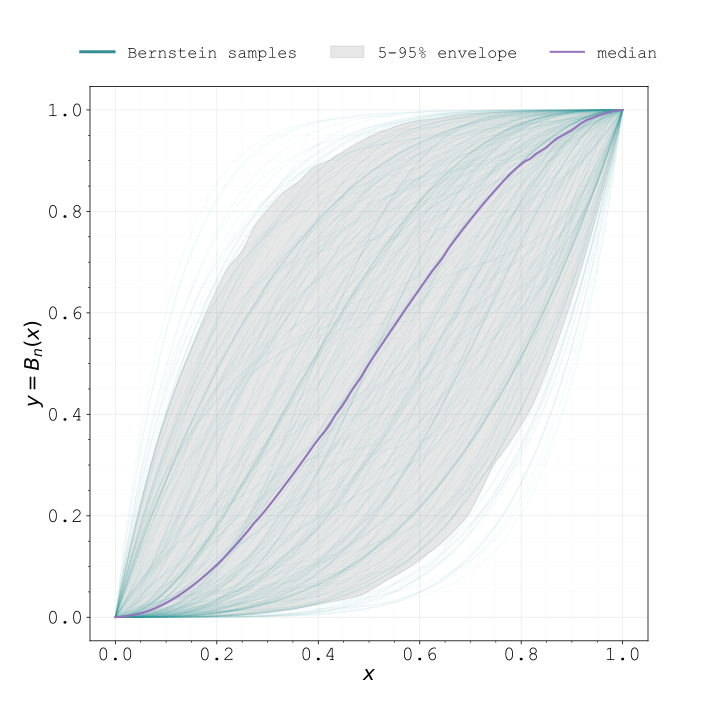
\includegraphics[width=\linewidth]{img/bernstein}
	\captionof{figure}{\centering Zufällige Bernsteinpolynome fungieren als verschiedene kumulative Verteilungsfunktionen für die probabilistischen opaken Prädikate.} %mit $k=0$ und $a=1$
	\label{fig:bernstein}
\end{minipage}

%Dadurch, dass $F$ monoton steigend ist, lässt sich $F$ als sortierte Liste an $y$-Werten betrachten. Das Inverse der kumulativen Verteilungsfunktion lässt sich folglich  über eine Binärsuche effizient in $\mathcal{O}(\log(n))$ wie folgt berechnen:
%Die Berechnung des Inversen der kumulativen Verteilungsfunktion geschieht über Binärsuche folgendermaßen:
Das Inverse der kumulativen Verteilungsfunktion lässt sich effizient über das Newton-Raphson-Verfahren mit Laufzeitkomplexität $O(k)$ berechnen, wobei $k$ die Anzahl an Iterationen festlegt\footnote{Hierfür muss das Bernsteinpolynom mit \emph{streng} monoton steigenden Koeffizienten (Mindestabstand) generiert werden.}. Aufgrund des quadratischen Konvergenzverhaltens des Verfahrens genügen für $64$-Bit Gleitkommazahlen praktisch $k=6$ Iterationen: Gemäß der IEEE 754 Norm haben $64$-Bit Gleitkommazahlen eine $52$-Bit Mantisse. Durch das Konvergenzverhalten verdoppelt sich die Anzahl korrekter Bits mit jeder Iteration. Ist anfänglich $1$ Bit korrekt erraten, so braucht es $6$ Iterationen, um alle $2^6=64>53$ Bits der Mantisse korrekt zu bestimmen. Um Sicherheitsgarantien zu liefern wurde der Algorithmus mit $k=7$ implementiert, um bei schlechten anfänglichen Schätzungen und ungünstigen Bernsteinpolynomen dennoch garantiert das Inverse der kumulativen Verteilungsfunktion korrekt zu bestimmen. Die zusätzlichen Laufzeitkosten hierdurch sind minimal. Um eine mögliche Divergenz des Newton-Raphson-Verfahrens zu verhindern, wird der geschätzte Wert bei jeder Iteration auf den Definitionsbereich $\mathbb{D}$ der Funktion begrenzt. Der Pseudocode hierfür ist in \cref{alg:invCumSum} gegeben.¸
\begin{algorithm}[!h] 
	\caption{Berechnung inverser kumulativer Verteilungsfunktion über das Newton-Raphson-Verfahren }
	\label{alg:invCumSum}
	\begin{algorithmic}[1]
		\Require $\Var{C}$ (Bernstein coefficients), $\Var{HShift}, \Var{VStretch}$ (horizontal shift/ vertical stretch), $\Var{Precision}$ (determines precision of Bernstein evaluation) %\textbf{as hardcoded constants}
		\Function{SampleBernsteinInverse}{$\Var{U} \in [0, 1]$}
		\State $\Var{Estimate} \gets \Var{HShift} + \frac{0.5}{\Var{VStretch}}$ \Comment{Start guess at center of domain.}
        
        \State $\Var{D_{start}} \gets \Var{HShift}$
        \State $\Var{D_{end}} \gets \Var{HShift} + \frac{1}{\Var{VStretch}}$
		
		\For{$i \gets 0$ \textbf{to} $\Var{Precision}$}
			\State $\Var{t} \gets \Var{VStretch} \cdot (\Var{Estimate} - \Var{HShift})$ \Comment{Transformed $\Var{Estimate}$.}
			\State $\Var{y} \gets 0.0$ \Comment{Accumulator for $B(t)$.}
			\State $\Var{y'} \gets 0.0$ \Comment{Accumulator for $B'(t)$.}
			
			\For{$\Var{k} \gets 0$ \textbf{to} $\Var{Degree}$} \Comment{Evaluate CDF $B(t)$}
			\State $\Var{b_{k}} \gets \binom{n}{k} \cdot t^k \cdot (1-t)^{n-k}$ 
			\State $\Var{y} \gets \Var{y} + \Var{C}[k] \cdot \Var{b_{k}}$
			\EndFor
			
			\For{$\Var{k} \gets 0$ \textbf{to} $\Var{Degree}-1$} \Comment{Evaluate PDF.}
			\State $\Var{b'_{k}} \gets \binom{n-1}{k} \cdot t^k \cdot (1-t)^{n-1-k}$ 
			\State $\Var{y'} \gets \Var{y'} + \Var{C'}[k] \cdot \Var{b'_{k}}$
			\EndFor
			
			\State $\Var{OffsetY} \gets \Var{y} - \Var{U}$
			\State $\Var{Slope} \gets \Var{y'} \cdot \Var{HStretch}$ \Comment{Apply chain rule: $\frac{dy}{dx} = \frac{dy}{dt} \cdot \frac{dt}{dx}$.}
			
			\State $\Var{Estimate} \gets \Var{Estimate} - \frac{\Var{OffsetY}}{\Var{Slope}}$ \Comment{Newton Step.}
            
            \State $\Var{Estimate} = \Call{max}{\Call{min}{\Var{Estimate}, \Var{D_{start}}}, \Var{D_{end}}}$ \Comment{Clamp to prevent divergence.}
		\EndFor
		
		\State \Return $\Var{Estimate}$
		\EndFunction
	\end{algorithmic}
\end{algorithm}

\subsection{Generierung von Pseudozufallsvariablen} \label{sec:pseudoZufall}
Damit der vorgestellte Ansatz funktionieren kann, bedarf er einer gleichverteilten (Pseudo-)Zufallszahl, welche auf dem Einheitsintervall liegt und zugleich als unbestimmte symbolische Variable ohne konkreten Wert von symbolischen Ausführungsengines betrachtet wird.
%Hierfür kommen infrage:
%\begin{enumerate}[]
%    \item Betriebssystem- (z.B. \texttt{rand() oder \texttt{time()}}) und Hardware-APIs (z.B. \texttt{rdtsc}), 
%    \item die Zufallszahlgenerierung mittels Race Conditions \cite{colesaRandomRace} oder
%    \item die Nutzung von Funktionsparametern, deren Werte sich nicht statisch festlegen lassen (\emph{Parameter Sampling}).
%\end{enumerate}
%
%In Fällen 1-2 sind die genutzten Quellen nach erstmaliger Bestimmung leicht wiedererkennbar. Dies erleichtert für Angreifer die Suche nach probabilistischen opaken Prädikaten und mindert folglich auch ihre Tarnung.
%Es wurde sich daher für Methode 3 entschieden: ein zufälliger Funktionsparameter wird für jede zu obfuskierende Funktion ausgewählt und auf dem Einheitsintervall $[0;1]$ abgebildet.
Hierfür wird für jede zu obfuskierende Funktion ein zufälliger Funktionsparameter ausgewählt und auf dem Einheitsintervall $[0;1]$ abgebildet.
%In der Praxis können Angreifer kaum ganze Programme symbolisch auszuführen, sondern immer nur einzelne Funktionen. Je größer der Abschnitt, welcher symbolisch ausgeführt wird, desto höher die Wahrscheinlichkeit, dass nicht implementierte Nebenwirkungen die Ergebnisse verfälschen, es zu einer Zustandsraum-Explosion (\emph{State Space Explosion}) kommt oder das \emph{Constraint Solving} sich aufgrund seiner exponentiellen Laufzeitkomplexität nicht mehr in vertretbarer Zeit durchführen lässt \cite{baldoniSurveySymbolicExecution2018}. Dies bedeutet, dass der Parameter vom \emph{Constraint Solver} als unbestimmte symbolische Variable behandelt werden muss. 
Hierdurch sind die opaken Prädikate gut getarnt -- ein Parameterzugriff ist schließlich normales Verhalten in jedem Programm. Die einzige Gefahr ist dabei, dass der gewählte Parameter immer konstante Werte annimmt. Ein Angreifer könnte in diesem Fall alle Werte dieses Parameters in Funktionsausrufen sammeln und die Funktion mit ihnen ausführen. Sind für jeden Parameterwert die ausgeführten Basisblöcke gleich, so handelt es sich bei den nicht ausgeführten Basisblöcken um "`Junkcode"'. Prädikate, welche auf diese Basisblöcke verweisen sind folglich opak und können gelöscht werden. \textbf{Diese Vulnerabilität wurde in keiner der gelesenen Arbeiten zum Thema bis jetzt angesprochen.} \cref{alg:symVar} bietet hierfür eine Lösung.
\begin{algorithm}[!h] 
    \caption{Suche nach Parameter mit extern-abgeleiteten Wert in Funktionsaufruf über DFS}
    \label{alg:symVar}
    \begin{algorithmic}[1]
        \Function{GetSymbolicVariable}{$Function \; \Var{F} \in \Var{Module}$}
            \ForAll{$Callsite \; \Var{CS} \in \Var{F}$}
                \ForAll{$Argument \; \Var{Arg} \in \Var{CS}$}
                    \State $\Var{Visited} = \Var{HashMap()}$
                    
                    \If{$\Call{IsVariableDerivedFromExternal}{\Var{Arg}, \Var{Visited}}$}
                        \Return $\Var{Arg}$
                    \EndIf
                \EndFor
            \EndFor
        \EndFunction
        
        \\
        
        \Function{IsDerivedFromExternal}{$Argument \; \Var{Arg}, Hashmap \; \Var{Visited}, \Var{Depth} \in \mathbb{Z}$}
            \If{$\Var{Depth} > 30 \vee \Var{Arg} \in \Var{Visited}$} 
                \Return \False \Comment{Constant was deemed empirically suitable.}
            \EndIf
            
            \State $\Var{Visited}[\Var{Arg}] = \textbf{true}$
            
            \If{$\Var{Val}$ is result of {External Function}}
                \Return \True \Comment{Check immediate origin}
            \EndIf
            
            \If{$\Var{Val}$ is {Internal Function Call}} \Comment{Determine data sources $\mathcal{S}$ based on operation type}
                \State $\mathcal{S} \gets$ Return statements of the called function
            \ElsIf{$\Var{Val}$ is {Memory Read}}
                \State $\mathcal{S} \gets$ Values written to the source address (by Stores)
            \Else \Comment{Arithmetic, Casts, PHI inputs}
                \State $\mathcal{S} \gets$ $\Var{Val}.Operands$ 
            \EndIf
            
            \ForAll{$\Var{Src} \in \mathcal{S}$} \Comment{Recursively trace data flow}
                \If{$\Call{IsDerivedFromExternal}{\Var{Src}, \Var{Visited}, \Var{Depth} + 1}$}
                    \Return \True
                \EndIf
            \EndFor
            
            \State \Return \False
        \EndFunction
    \end{algorithmic}
\end{algorithm}
%\subsection{Füllcode}
%\textcolor{red}{TODO: entfernen?}
%Ohne gut getarnten Füllcode ist eine Erkennung des unwahrscheinlichen Prädikats trivial. Der Pfad, welcher die plausibelsten Anweisungen enthält ist der Richtige, unabhängig von der Qualität des opaken Prädikats. 
%Da diese Arbeit nicht das Ziel hat, qualitativ hochwertigen Füllcode zu generieren, wird für den unwahrscheinlicheren Prädikatwert der Kontrollfluss auf ein zufälligen Basisblock der zu obfuskierenden Funktion übertragen. %Hierdurch erscheinen beide Pfade ausgehend vom Prädikat für einen Angreifer plausibel.
%Für den Machbarkeitsnachweis dieser Arbeit genügt dies. Eine für den Praxisgebrauch bestimmte Implementierung müsste dies mit den dargelegten Methoden anderer Arbeiten ergänzen.

\section{Implementierung} \label{sec:implementierung}
%\subsection{Entscheidungen}
Zur Implementierung wurden drei Ansätze erwogen: die Entwicklung eines Bin2Bin-Obfuskators\footnote{Direkte Manipulation von Assembler-Anweisungen existierender Programme.}, die Implementierung in Form eines LLVM-Passes \cite{LLVM, LLVMProject}\footnote{Nutzung des LLVM-Projekts, um einen sog. \emph{Compiler-Pass} zu schreiben.} sowie die Quellcodemanipulation\footnote{durch z.B. C-Makros und das Einfügen von inline Assembler-Ausschnitten}
Es wurde eine Entscheidung für einen LLVM-Pass getroffen aufgrund folgender Vorteile:
\begin{enumerate}[]
    \item \textbf{Abstraktion und Portabilität:} LLVM entkoppelt durch eine abstrakte Zwischensprache (\emph{Intermediate Representation}) von Architektur-/Betriebssystemdetails. Viele \emph{low-level} Aufgaben (z.B. \emph{Relocations}, Einfügen von Assembler-Anweisungen etc.) werden übernommen.
    \item \textbf{Optimierung:} Die LLVM-Toolchain enthält etablierte Optimierungs-Pässe und profitiert fortlaufend von der Arbeit zahlreicher Beiträgender. Dies ermöglicht eine nahezu optimale Kompilation obfuskierter Programme, welche sich als nützlich und sogar erforderlich in vielen Anweundungssituationen erweist (z.B. \emph{Embedded Systems}, IoT, Echtzeitsysteme etc.).
    \item \textbf{Entwicklungsaufwand:} Bin2Bin-Obfuskatoren und umfangreiche Quellcodemanipulation erfordern viel manuellen Aufwand und sind fehlerhaftig. Ein LLVM-Pass ermöglicht den reinen Fokus auf die Obfuskationslogik.
\end{enumerate}
%\begin{figure}[h]
%    \centering
%    \includegraphics[width=0.8\linewidth]{img/llvm-pass}
%    \caption{Schematische Darstellung eines LLVM-basierten Build-Prozesses mit optionalem Obfuskator-Pass.}
%    \label{fig:llvm-pass}
%\end{figure}
Ein LLVM-Pass bietet in diesem Fall das beste Kompromissverhältnis zwischen \emph{low-level} Kontrolle, Laufzeiteffizienz, einer \emph{high-level} Portabilität sowie vertretbarem Entwicklungsaufwand.

Der Pass wurde mit mehreren Parametern versehen (vgl. \cref{alg:bashScript}): Nutzer können angeben, wie viel Prozent der Funktionen obfuskiert werden sollen (\texttt{-pop-lvl}), wie wahrscheinlich die probabilistischen opaken Prädikate sein sollen (\texttt{-pop-pred-prob}) sowie den minimalen/maximalen Bernsteinpolynomgrad (\texttt{-pop-min}/\texttt{max-degree}).
Zudem können Funktionen im Quellcode als zu obfuskierend markiert werden (vgl. \cref{alg:toObf})
%Da in der Implementierung alle Zufahlszahlen vom selben PRNG generiert werden, kann der anfängliche Startwert (\emph{Seed}) als Schlüssel für die Obfuskation betrachtet werden.

Die Implementierung, Beispiele und Experimente sind unter \cite{paulPOP} veröffentlicht.
%\textcolor{red}{TODO: Inspiration von ogisoSoftwareObfuscationTheoretical2003 nehmen!}
\begin{figure}[!h]
	\centering 
	\label{fallbsp}
	\begin{minipage}[c]{0.36\textwidth}
		\begin{subfigure}[b]{\linewidth}
			\begin{lstlisting}[style=customc_compact, captionpos=b, language=bash]	
#!/bin/bash

OPT_LVL=O3
FILENAME="hello_world"
PASS_PLUGIN_DIR="Obfuscator.so"
LVL=50 RUNS=1 PRED_PROB=99
MIN_DEG=3 MAX_DEG=6

clang -$OPT_LVL \
-fpass-plugin=$PASS_PLUGIN_DIR \
-Xclang -load -Xclang $PASS_PLUGIN_DIR \
-mllvm -pop-lvl=$LVL \
-mllvm -pop-pred-prob=$PRED_PROB \
-mllvm -pop-runs-per-fn=$RUNS \
-mllvm -pop-min-degree=$MIN_DEG \
-mllvm -pop-max-degree=$MAX_DEG \
${FILENAME}.c \
-o $FILENAME\end{lstlisting}
            \vspace*{-22pt}
			\caption{Bash-Skript zur Ausführung der implementierten Obfuskation auf C(++) Quellcode.}
            \label{alg:bashScript}
		\end{subfigure}
		
		\vspace{1em}
		
		\begin{subfigure}[b]{\linewidth}
			\begin{lstlisting}[style=customc_compact, captionpos=b]	
__attribute__(annotate("POP"))
void foo(int x)
{
	printf("foo %i\n", x);
}			\end{lstlisting}
            \vspace*{-22pt}
			\caption{Eine einfache zu obfuskierende Funktion.}
			\label{alg:toObf}
		\end{subfigure}
	\end{minipage}
	\hfill
	\begin{minipage}[c]{0.6\textwidth}
		\begin{subfigure}[c]{\linewidth}
            \setstretch{0.9} 
			\begin{lstlisting}[style=customc_compact, captionpos=b, firstnumber=1]
void __fastcall foo(uint64_t x)
{
	__m128d v7;
	uint64_t v8 = x;
	double v9 = x * COERCE_DOUBLE(0x4000000000000LL);
	double v10 = 35.31442506435751;
	for ( i = 0; i != 7; ++i )
	{
		__m128d v1 = *&v10;
		double v6 = (v10 - 35.29940863512881) * 33.29686388054899;
		v1.m128d_f64[0] = v10 - (0.0 * ((1.0 - v6) * (1.0 - v6) * (1.0 - v6)) + 0.5018965731323943 * v6 * ((1.0 - v6) * (1.0 - v6)) + 1.199789464169086 * (v6 * v6) * (1.0 - v6) + v6 * v6 * v6 - v9) / ((0.5018965731323943 * ((1.0 - v6) * (1.0 - v6)) + 1.395785782073383 * v6 * (1.0 - v6) + 1.800210535830914 * (v6 * v6)) * 33.29686388054899);
		v7 = v1;
		v2 = _mm_cmplt_sd(0x4041AA2B238C72F8uLL, v1);
		v3 = _mm_or_pd(_mm_andn_pd(v2, v1), _mm_and_pd(v2, 0x4041AA2B238C72F8uLL));
		v4 = _mm_cmplt_sd(v3, 0x4041A65305AC0256uLL).m128d_f64[0];
		*&v10 = ~*&v4 & *&v3.m128d_f64[0] | *&v4 & 0x4041A65305AC0256LL;
	}
	if ( v7.m128d_f64[0] <= 35.32927409341327 )
		printf("foo %lu\n", *(&v5 - 2)); // This Basic Block will always be executed.
	else
		// Junkcode; This Basic Block will never be executed
}			\end{lstlisting}
            \vspace*{-22pt}
			\caption{Dieselbe Funktion aber mit PoP (Bernsteinpolynomgrad $n=3 $) obfuskiert. Pseudo-C wurde modifiziert aus der Dekompilation von IDA entnommen. Die Funktionen mit dem Unterstrich als Präfix sind intrinsische Funktionen. Sie kapseln einzelne CPU-Anweiseungen.}
			\label{alg:doneObf}
		\end{subfigure}
	\end{minipage}
%    \vspace*{-10pt}
%    \caption{Fallbeispiel zur Obfuskation von C(++)-Programmen.}
\end{figure}

\section{Evaluierung} \label{sec:evaluierung}
\subsection{Vorgehen} \label{sec:kriterien}
Für die Evaluierung wurden die weitverbreiteten Kriterien von Collberg et al. \cite{collbergATaxonomyOfObfuscatingTransformations} verwendet\label{par:metriken}:
\begin{center}
    \begin{tabular}{c|l}
    	\textbf{Kriterium} & \textbf{Beschreibung} \\
        \hline
        Kosten & Wie sehr erhöht die Obfuskation die Laufzeitkosten? \\
    	\hline
    	Stärke & Wie unverständlich ist das obfuskierte Programm für einen Angreifer? \\
    	\hline
    	Resilienz & Wie schwer ist eine (automatisierte) Deobfuskation? \\
    	\hline
    	Tarnung & Wie auffällig ist die Obfuskation? %Wie leicht lässt sich ein obfuskiertes Programm als solches erkennen? \\
    \end{tabular}
\end{center}
%Die Obfuskationsmethode wurde dabei auf Programme aus \cite{banescuCodeObfuscationSymbolic2016}\footnote{\url{https://github.com/tum-i4/obfuscation-benchmarks}}, auf mehrere Verschlüsselungs-/Hashverfahren (AES, DES, MD5, RC4 \& SHA1.) von \cite{ollivierHowKillSymbolic2019a} sowie auf die GNU Core Utilities angewandt. Insgesamt wurden somit über \textcolor{red}{TODO} Programme obfuskiert. Die Programme wurden bewusst gewählt, um typische realistische Szenarien abzubilden, in denen z.B. kryptographische Algorithmen zum Schutz geistigen Eigentums eingesetzt werden \cite{schloegelTechnicalReportHardening2022}.
Es wurde sich bewusst gegen die einfachen Benchmarkprogramme wie in \cite{banescuCodeObfuscationSymbolic2016, obfuscatorBenchmarks} oder \cite{ollivierHowKillSymbolic2019a} entschieden. Orientiert wurde sich dabei am zur Zeit umfangreichsten Literaturreview zur (De-)Obfuskation \cite{sutterEvaluationMethodologiesSoftware2024}. Dieses bemängelt mangelnde Programmgröße sowie -quantität in der aktuellen Obfuskationsforschung. Es wurde sich daher für die LLVM Test Suite \cite{llvmTestSuite2025} entschieden. Dabei wurde sich auf die größten vollständigen Anwendungen (darunter z.B. SQLite \& Lua) und Benchmarkprogramme der \texttt{MultiSource} Untereinheit (31 Programme) beschränkt.
Obwohl die Test Suite eigentliche für Compilerevaluierungen entwickelt wurde, ist sie dennoch für die Obfuskationsevaluierung geeignet, da sie durch ihre diversen Programme realistische Anwendungsszenarien der Obfuskation abbildet.
Die Test Suite bietet zudem den Vorteil vorgefertigter Tests (167 Tests), welche die Korrektheit obfuskierter Programme prüfen.

Alle Programme wurden mit clang 18.1.3 und Optimierungslevel \texttt{-O3} kompiliert und mit Ubuntu 24.04.3 LTS mit Kernel Version 5.16, einer Intel\textregistered \;Core\texttrademark \;i7-10700F CPU und $16$Gb DDR4 RAM ausgeführt.
Es wurden dabei $k=8$ Newton-Raphson-Iterationen gewählt, $n=4$ als durchschnittlichen Bernsteinpolynomgrad sowie Erfolgswahrscheinlichkeit $P(\Var{RealBB})=1-10^{-5}$ verwendet. Jede Funktion bekommt dabei maximal ein probabilistisches opakes Prädikat. Benchmarks und Auswertungsskripts sind unter \cite{paulPOP} verfügbar.

\subsection{Evaluierung}
\subsubsection{Kosten}
\begin{minipage}[t]{0.49\textwidth}
	\centering
	\includegraphics[width=1\textwidth]{img/stats/compilation_time}
	\captionof{figure}{\centering Durchschnittliche Kompilationszeit in Abhängigkeit vom Obfuskationslevel}
	\label{fig:compilationTime}
\end{minipage} \hfill
\begin{minipage}[t]{0.49\textwidth}
	\centering
	\includegraphics[width=1\textwidth]{img/stats/size}
	\captionof{figure}{\centering Programmgröße in Abhängigkeit vom Obfuskationslevel}
	\label{fig:size}
\end{minipage}
\begin{minipage}[t]{0.49\textwidth}
	\centering
	\includegraphics[width=1\textwidth]{img/stats/runtime}
	\captionof{figure}{\centering Laufzeit in Abhängigkeit vom Obfuskationslevel}
	\label{fig:runtime}
\end{minipage}
\begin{minipage}[t]{0.49\textwidth}
	\centering
	\includegraphics[width=1\textwidth]{img/stats/pass_rate}
	\captionof{figure}{\centering Testerfolg in Abhängigkeit vom Obfuskationslevel}
	\label{fig:passRate}
\end{minipage}
\\\\
Um die Obfuskationskosten zu messen wurden die durchschnittliche Programmgröße (\cref{fig:size}), -laufzeit (\cref{fig:runtime}), Kompilationszeit (\cref{fig:compilationTime}) und Erfolgsquote (\cref{fig:passRate}) von 5 Kompilationen der gesamten LLVM Test Suite erhoben. Alle Messgrößen wurden test-weise relativ zu Obfuskationslevel 0 normalisiert.

Die Kompilationszeit wächst linear mit der Obfuskationsrate, wie sich \cref{fig:compilationTime} entnehmen lässt.
%Die größten Auswirkungen hatte die Obfuskation auf die Programmlaufzeit (\cref{fig:runtime}).
%Die medianen Laufzeitkosten steigen hier von \textcolor{red}{TODO} auf $\sim1,12$ der Laufzeit unobfuskierter Programme. Der Median der Programmgröße steigt bis etwa 1,23. Beides deutet darauf, dass der typische Overhead begrenzt bleibt.
%Die Quantile \textcolor{red}{TODO}.
%%\textcolor{red}{TODO: Auf Median, Quartile 2x eingehen.}
%Auffällig ist dabei die große Distanz zwischen Minima und Maxima. Die Maxima lassen sich durch die kleineren Programme der Test-Suite erklären, auf welche die Obfuskation eine verhältnismäßig größere Auswirkung hat. Warum manche Programme nach der Obfuskation sogar schneller sind, ist unklar. Das Verhalten wurde bereits bei komerziellen Obfuskationsprodukten beobachtet\cite{codedefenderMetrics}.

Wie zu erwarten war zeigt sich ein direkter Zusammenhang zwischen Obfuskationslevel und Code-Größe (\cref{fig:size}). Während der Median moderat auf ca. 1,25 ansteigt, wächst die Varianz signifikant an. Bei 100\% Obfuskation erreichen die Spitzenwerte mehr als das Doppelte ($\sim2,2$) der Ursprungsgröße. Der Anstieg wird durch das obere Quartil (Q3) getrieben. Während das untere Quartil (Q1) nahe 1,1 verharrt (es gibt also Fälle mit minimalem Overhead), steigt Q3 bei 100\% Obfuskation auf ca. 1,6 an. Dass die untere Antenne bis 1,0 reicht ist darauf zurückzuführen, dass sich in 2 Fällen aufgrund fehlender Funktionsparameter keine probabilistischen opaken Prädikate einfügen ließen. Um dies zu korrigieren müsste die Implementierung des Obfuskators zukünftig mit Parameter-Insertion erweitert werden. 

Bei der Laufzeit bleibt der Median stabil nahe 1,1, welches auf geringe durchschnittliche Laufzeitkosten hindeutet. Die Streuung (Interquartilsabstand und Minimum/Maximum) nimmt bei höheren Obfuskationsleveln stark zu: 25\% der Programmausführungen benötigen die doppelte Laufzeit oder mehr. Die Maxima bei Größe/Laufzeit lassen sich durch die kleineren Programme der Test-Suite erklären, auf welche die Obfuskation eine verhältnismäßig größere Auswirkung hat. Warum manche Programme nach der Obfuskation sogar schneller sind, ist unklar. Das Verhalten wurde bereits bei komerziellen Obfuskationsprodukten beobachtet\cite{codedefenderMetrics}.

Die sich in der Größe oder Laufzeit ergebenden Kosten lassen sich beide durch ein Finetuning der Obfuskatoreinstellungen vermindern, z.B. indem nur bestimmte Funktionen obfuskiert bzw. performance-kritische Funktionen nicht obfuskiert werden.

Hervorzuheben ist, dass trotz der geringen Wahrscheinlichkeit, dass die probabilistischen opaken Prädikate versagen, auch größere Projekte wie SQLite problemlos kompilieren und fehlerfrei funktionieren (\cref{fig:passRate}).
%\textcolor{red}{Der Abnehmende Testerfolg  in \cref{fig:passRate} liegt an den für die Tests als Fehler geltenden unerwarteten Gleitkommazahl-Flagänderungen. Die vermeintlichen fehlerhaften Programme wurden geprüft und problemlos manuell ausgeführt. Die vorgefertigten Tests sind lediglich zu streng.}
Insgesamt sind die Kosten je nach Programm/Anwendungsfall und Obfuskationslevel praxisgerecht.

\subsubsection{Stärke} \label{sec:stärke}
Wie in \cite{xuManufacturingResilientBiOpaque2018} angemerkt wurde, ergibt eine Quantifizierung von Stärke bei der Evaluierung neuer opaker Prädikate wenig Sinn. Relevante Metriken wie die zyklomatische Komplexität (McCabe-Metrik) erhöhen sich beliebig mit der Häufigkeit opaker Prädikate und nicht durch ihre Art.

Auf qualitativer Ebene lässt sich anmerken, dass probabilistische opake Prädikate indirekt auch die Schwachstellen der Analysewerkzeuge heutiger Angreifer angreifen. 
Konkret sind moderne Dekompilierer wie IDA/Binary Ninja/Ghidra noch nicht in der Lage, bestimmte SIMD (\emph{Single Instruction, Multiple Data})-Anweisungen zu dekompilieren.
Dies lässt sich an \cref{alg:doneObf} erkennen, wo IDA die unbekannten Anweisungen durch intrinsische Funktionen darstellt anstelle von verständlicherem Pseudo-C.
Experimente mit \emph{Decompiler Explorer} \cite{vec35DecompilerExplorer} zeigen, dass keine der aktuellen \emph{State-of-the-Art}-(SOTA)-Dekompilierer bis auf Ghidra in der Lage ist, die SIMD Anweisungen in Pseudo-C zu dekompilieren. Durch eine Feinjustierung der clang Kommandozeilenoptionen nutzten die probabilistischen opaken Prädikate AVX-512 Anweisungen. Hierdurch konnten die Dekompilierer noch weniger in Pseudo-C dekompilieren. Die Nutzung der \emph{Decompiler Explorer}-Website war hiernach nicht mehr möglich. Diese Limitation bedeutet für Angreifer, dass eine Verständnis der Obfuskation (und somit auch der Programmlogik) mehr Zeit, Aufwand und vor allem ein Verständnis von Assembler erfordert. Die Hürde zum erfolgreichen Reverse-Engineering ist somit erhöht.

\subsubsection{Resilienz}
Da sich die Resilienz im Falle dieses Projekts nicht quantitativ messen lässt, wird sie qualitativ untersucht.
Hierfür wurden folgende Angriffsmethoden auf das einfache Programm aus \cref{fallbsp} sowie die 5 Sortieralgorithmen aus \cite{banescuCodeObfuscationSymbolic2016, obfuscatorBenchmarks} angewandt\footnote{Gelangt es den symbolischen Ausführungsengines bei diesen einfachen Programmen nicht, den richtigen Basisblock zu erkennen, kann dies bei größeren Programmen auch nicht geschehen.}: 
\begin{itemize}
	\item Symbolische Ausführung mit Angr \cite{shoshitaishvili2016state} (v.9.2.189),
    \item Triton \cite{SSTIC2015-Saudel-Salwan} (v.1.0.0rc4) und
    \item Binsec (v.0.11.0) \cite{binsec2020}
    %Miasm \cite{desclaux2018miasm} (v.0.1.5)
%	\item Programmsynthese mittels Syntia \cite{blazytkoSyntiaSynthesizingSemanticsa} (commit 3602893) und Xyntia \cite{menguySearchBasedLocalBlackBox2021} (commit 7b20733)
%    \item Programmsynthese mittels Xyntia \cite{menguySearchBasedLocalBlackBox2021} (commit 7b20733)
%	\item Probabilistische Analyse über mehrfache Ausführung obfuskierter Programme mit zufälligen Werten \cite{dallapredaOpaquePredicatesDetection2006}
\end{itemize}
Wie vermutet waren keine der symbolischen Ausführungsengines in der Lage, die Möglichkeit, dass einer der zwei Pfade nie ausgeführt wird, auszuschließen. 
Alle drei symbolischen Ausführungsengines erkannten entweder wie hypothetisiert beide Basisblöcke ausgehend vom Prädikat als möglich (Binsec), hängten und konnten nicht innerhalb von 8 Stunden die Constraints des unwahrscheinlichen Pfades extrahieren (Angr) oder konnten gar keine Constraints extrahieren (Triton) (vgl. \cref{tab:symexec}).

\begin{table}[ht]
    \centering
    \begin{tabular}{l l l l}
        \toprule
        \textbf{Engine/Solver} & \textbf{Version} & \textbf{Ergebnis}\\
        \midrule
        Angr (Z3) & 9.2.189 & \ding{54} keine Constraint-Extraktion (Abbruch nach 8h) \\%& 8\,h 
        Triton (Z3) & 1.0.0rc4 & \ding{54} keine Constraints gefunden \\%& <1\,s 
        Binsec (Bitwuzla)  & 0.11.0 & \ding{54} Beide Basisblöcke sind erreichbar \\%& 21\,min 
        \bottomrule
    \end{tabular}
    \caption{Ergebnisse der symbolischen Ausführung.}
    \label{tab:symexec}
\end{table}

Eine probabilistische Analyse über mehrfache Ausführung obfuskierter Programme mit zufälligen Werten \cite{dallapredaOpaquePredicatesDetection2006} erkennt zwar die probabilistischen opaken Prädikate und die korrekten Basisblöcke, markiert aber auch hier fälschlicherweise $20-40\%$ regulärer Prädikate der untersuchten Programme als opak.
%Wie in \cite{dallapredaOpaquePredicatesDetection2006} empirisch untersucht, markiert eine probabilistische Analyse auch hier fälschlicherweise $20-40\%$ regulärer Prädikate der untersuchten Programme als opak. \textcolor{red}{TODO: Standardabweichung}
Dies ist damit zu begründen, dass auch viele Prädikate der unobfuskierten Programmlogik besonders häufig gleiche Werte annehmen.

Trotzdem ist eine Deobfuskation theoretisch möglich. Erkennt ein Angreifer ein Prädikat als opak, so muss er nur über dynamischer Ausführung den korrekten Pfad bestimmen. Die Resilienz der Obfuskation basiert somit auf dessen Tarnung. Wie \cref{sec:tarnung} zeigt ist eine wiederholte automatisierte Erkennung bei einer Kombination mit anderen Obfuskationsmethoden allerdings schwierig.

Zudem ist eine Anwendung von an die Obfuskationsmethode angepassten Heuristiken möglich. Ein Angreifer könnte z.B. alle Prädikate mit symbolischen Ausführungsengine ausführen und die benötigte Zeit für die Extraktion der Constraints beider Pfade messen. Dauert dies für einen Pfad länger als eine festgelegte konstante Zeit, so handelt es sich mit hoher Wahrscheinlichkeit um ein probabilistisch opakes Prädikat. Trotzdem hat die Methode denselben Nachteil wie die probabilistische Analyse -- ihre Korrektheit ist nie garantiert.

\subsubsection{Tarnung} \label{sec:tarnung}
\begin{figure}[!h]
    \centering
    \includegraphics[width=0.6\textwidth]{img/stats/stealth}
    \centering
    \caption{\centering Histogramm und KDE der Wahrscheinlichkeitsdichte der euklidischen Distanz zum Mittelpunkt unobfuskierter Prädikate vor/nach der Obfuskation} 
    \label{fig:opcodeDist}
\end{figure}
\begin{table}[!h]
    \centering
    \footnotesize
    \renewcommand{\arraystretch}{0.9}
    \setlength{\tabcolsep}{4pt}
    \begin{tabularx}{1\textwidth}{@{}l >{\raggedright\arraybackslash}X@{}}
        \toprule
        \textbf{Kategorie} & \textbf{Anweisungen} \\
        \midrule
        Arithmetik & \texttt{imul, inc, sub, add, idiv, divsd, sbb, subpd, addpd, mulpd, divpd, maxpd, minpd, sqrtpd} \\
        Logik & \texttt{and, sar, xor, test, shr, shl, or, xorps, xorpd, orpd, andpd} \\
        Datenübertragung & \texttt{movaps, movsd, movabs, movzx, mov, movss, movsx, movsxd, stosd, movapd, movupd, unpcklpd, unpckhpd, movhpd, movlpd} \\
        Datenbreite/-konversion & \texttt{cvtss2sd, cvtsi2sd, cvtsd2ss, cqo, cdq, cvttsd2si} \\
        Zeigerarithmetik & \texttt{lea} \\
        Vergleich & \texttt{cmp, ucomisd, comisd} \\
        Sprünge & \texttt{jle, jne, jge, jae, jl, je, jg, jp, ja, jbe, jno, jmp} \\
        Stapel & \texttt{pop, push, call, ret} \\
        Boolesch & \texttt{setge, setne, setg, seta, setb, setl, sete} \\
        Sonstige & \texttt{nop} \\
        \bottomrule
    \end{tabularx}
    \caption{74 Assembler-Anweisungen in 10 Kategorien sortiert.}
    \label{tab:instrKategorien}
\end{table}

Um die Tarnung quantitativ zu messen wurde wie bei \cite{xuManufacturingResilientBiOpaque2018} vorgegangen. Hierfür wurden $n=4500$ jeweils unobfuskierte sowie obfuskierte Prädikate zufällig gewählt. Gemäß \cref{tab:instrKategorien} wurden die letzten zehn Anweisungen vor der bedingten Sprungsanweisung (inkl. der Sprunganweisung selbst) kategorisiert. Hierdurch kann jedes Prädikat $i$ als $10$-dimensionaler Vektor $\vec{x}_i$ dargestellt werden, wobei jede Dimension der absoluten Häufigkeit einer Anweisungskategorie in den letzten $10$ Anweisungen vor der Sprunganweisung entspricht. Um den Unterschied zwischen obfuskierten und unobfuskierten Prädikaten zu messen wurde zuerst der Mittelpunkt $\vec{m}=\frac{\sum_{i=1}^{n}{\vec{x}_i}}{n}$ aller unobfuskierten Prädikate berechnet. Die durchschnittliche Euklid'sche Distanz der obfuskierten Prädikate zum Mittelpunkt $\vec{m}$ entspricht ihrer Ähnlichkeit und somit auch Tarnung. Je geringer der Unterschied ist, desto höher die Tarnung.

Wie \cref{fig:opcodeDist} zu entnehmen ist, liegt die durchschnittliche Euklid'sche Distanz probabilistischer opaker Prädikate zu $\vec{m}$ bei $4,18$. Die durchschnittliche Distanz regulärer Prädikate zu $\vec{m}$ liegt bei $2,61$.
Die Distanz ist vor allem bei Programmen mit nur wenigen Gleitkommazahlberechnungen hoch. Die Tarnung lässt sich hier erhöhen durch eine Kombination mit anderen Obfuskationsmethoden, z.B. dem Einfügen von "`Dead Code"'/"`Junk Code"' mit vielen Gleitkommazahloperationen. 

Eine automatisierte Erkennung mittels Pattern-Matching erwies sich empirisch als schwierig. Es konnten keine Patterns erstellt werden, welche alle probabilistisch opaken Prädikate abdeckten. %Pattern Matching basierte Angriffe können zudem über die Anwendung von \emph{Mixed Boolean Arithmetic} Obfuskation verhindert werden. \textcolor{red}{TODO: Warum?}
Eine weitere Härtung ist über die Anwendung von \emph{Mixed Boolean Arithmetic} (MBA) Obfuskation auf das gesamte Programm möglich. Eine automatisierte Erkennung wird hier über die variablen Ausdrücke verhindert. Eine manuelle Erkennung der opaken Prädikate durch Angreifer ist behindert durch die Ununterscheidbarkeit der MBA Ausdrücke in den probabilistischen opaken Prädikaten vom Rest der obfuskierten Ausdrücke des Programms.

%Nicht gemessen wurde die Möglichkeit, über Machine Learning Methoden wie \cite{tofighi-shiraziDefeatingOpaquePredicates2019}, die opaken Prädikate wiederzuerkennen oder sogar zu deobfuskieren. 

\section{Fazit} \label{sec:fazit}
In der vorliegenden Arbeit wurde das neue Softwareobfuskationskonzept der probabilistischen opaken Prädikate eingeführt und in einer Implementierung in Form eines LLVM-Passes ein Machbarkeitsnachweis geliefert. Empirische Untersuchungen bestätigen, dass die vorgestellte Idee hinsichtlich ihrer Kosten, Resilienz, Stärke und Tarnung je nach Anwendungsfall und Kombination mit anderen Obfuskationsmethoden praxisgerecht ist. Dabei konnte nebenbei ein undokumentierter Angriffsvektor erkannt und eine Lösung dafür geboten werden.

Die Resilient probabilistischer opaker Prädikate gegen symbolische Ausführung wurde theoretisch und praktisch begründet. Praktische Untersuchungen zeigen zudem eine Resilienz gegen weitere Angriffsmethoden, wie die Programmsynthese, eine probabilistische Analyse sowie Pattern-Matching. Die Forschungsfrage ist somit positiv beantwortet.

Offen bleibt die Resilienz gegenüber Machine Learning basierten Deobfuskationattacken wie \cite{tofighi-shiraziDefeatingOpaquePredicates2019}. Auch mögliche Symbiosen mit verschiedenen Obfuskationsmethoden sollten weiter untersucht werden.
Gegenstand einer weiterführenden Auseinandersetzung sollte zudem die Anwendung der hier dargelegten Prinzipien der probabilistischen Obfuskation gegen andere Deobfuskationsmethoden. So könnte z.B. die Anwendung auf Ausdrücke Programmsynthesemethoden \cite{blazytkoSyntiaSynthesizingSemanticsa, menguySearchBasedLocalBlackBox2021} verhindern.

%\textcolor{red}{Verbesserung durch Anwendung anderer Obfuskationsmethoden (z.B. MBAs, Junkcode)} \\
%\textcolor{red}{probabilistisch opake Prädikate mit $P(\Var{RealBB})=0.5$ und zwei semantisch equivalenten aber unterschiedlich aussehenden Basisblöcken eingefügt} \\
%\textcolor{red}{Schlechtes Laufzeitverhalten relativieren} \\

\newpage

\section*{Danksagung}
Ich danke meinem schulischen Projektbetreuer, Herrn Dr. Arndt Latußeck für die wichtige Hinweisen zur Gliederung, Vorschläge zum Vorgehen bei der Evaluierung sowie der fachlichen Überprüfung der vorliegenden Arbeit. % Überprüfung meiner Forschungsfrage,

Zudem danke ich meiner Mutter, Claudia Baumgartner-Bardubitzki für ihre sprachliche Überprüfung.

Des Weiteren danke ich allen Entwicklern verschiedener Open-Source Softwarebibliotheken und -Anwendungen. Ohne diese wäre eine Ausarbeitung in der begrenzten Zeit und aktueller Form unmöglich gewesen.
\newpage

\pagenumbering{Alph}

\addcontentsline{toc}{section}{Literaturverzeichnis}
\printbibliography[title=Literaturverzeichnis]

\newpage

\addcontentsline{toc}{section}{Abbildungsverzeichnis}
\listoffigures

\end{document}